%-*- coding: UTF-8 -*-
% gougu.tex
% 勾股定理
\documentclass[UTF8] {ctexart}
\usepackage{graphicx}   % 为了使用插图功能
\usepackage{float}      % 用于设置浮动环境如table的参数
\usepackage{amsmath}    % 用于引用公式
\usepackage{geometry}   % 用于设计页面尺寸
\geometry{a6paper, centering, scale=0.8}    % 定义页面使用A6纸大小,版心居中,长宽占页面的0.8倍
\usepackage[format=hang, font=small, textfont=it]{caption}  % 用caption包改变图表标题格式
% 上面caption的设定是所有标题使用悬挂对齐方式(即编号向左突出),整体用小子号,而标题文本使用斜体(对汉字来说就是楷书)
\usepackage[nottoc]{tocbibind} % 增加目录的tocbibind包,默认会在目录中加入目录项本身、参考文献、索引等项目。
% 使用nottoc选项取消了在目录中显示目录本身

% 以下部分为导言区(preamble)一直到\begin{document}
\title{\heiti 杂谈勾股定理}
\author{\kaishu 张三}
\date{\today}
\bibliographystyle{plain}

% 可以在导言区定义新环境(newenvironment)和新命令(newcommond)来统一文章的格式,需要修改时,只要在导言区修改就可以了,而不必搜索全文。
\newenvironment{myquote}            % 定义新环境,名字为myquote
{\begin{quote}\kaishu\zihao{-5}}    % 环境开始处的代码,此处为使用楷书,字号为小五号
{\end{quote}}                       % 环境末尾处的代码,此处为空
\newcommand\degree{^\circ}           % 定义新命令,用\degree代替原来的角度

\begin{document}
\maketitle  % 输出论文标题,title、author、date并不马上出现在编译的结果中,而通过\maketitle排版
\begin{abstract}
这是一篇关于勾股定理的小短文。 % 摘要
\end{abstract}

\tableofcontents    % 输出目录

\section{勾股定理在古代}   % 开始新的一节
\label{sec:ancient}     % 给章节定义一个标签,{}里面的符号可以任取,但为了自动编号,不要用数字编号本身
西方称勾股定理为毕达哥拉斯定理,将勾股定理的发现归功于公元前 6 世纪的毕达哥拉斯学派 \cite{Kline}。该学派得到了一个法则,可以求出可排成直角三角
形三边的三元数组。毕达哥拉斯学派没有书面著作,该定理的严格表述和证明则见于欧几里德\footnote{欧几里德,约公元前 330--275 年。}《几何原本》
的命题 47:“直角三角形斜边上的正方形等于两直角边上的两个正方形之和。”证明是用面积做的。   % \footnote表示脚注
我国《周脾算经》载商高(约公元前 12 世纪)答周公问:
% \begin{quote}   % quote环境,引用一段话
% \zihao{-5}\kaishu 勾广三,股修四,径隅五。  % quote表示引用,\zihao{-5}表示字号为小5号,\kaishu表示字体为楷书
% \end{quote}
\begin{myquote}   % 用自定义的myquote环境,引用一段话
勾广三,股修四,径隅五。
\end{myquote}

又载陈子(约公元前 7--6 世纪)答荣方问:
% \begin{quote}
% \zihao{-5}\kaishu 若求邪至日者,以日下为勾,日高为股,勾股各自乘,并而开方除之,得邪至日。
% \end{quote}
\begin{myquote}
若求邪至日者,以日下为勾,日高为股,勾股各自乘,并而开方除之,得邪至日。
\end{myquote}
都较古希腊更早。后者已经明确道出勾股定理的一般形式。图\ref{fig:xiantu}是我国古代对勾股定理的一种证明 \cite{quanjing}。    % \cite表示引用,参考文献数据库在math.bib里
% 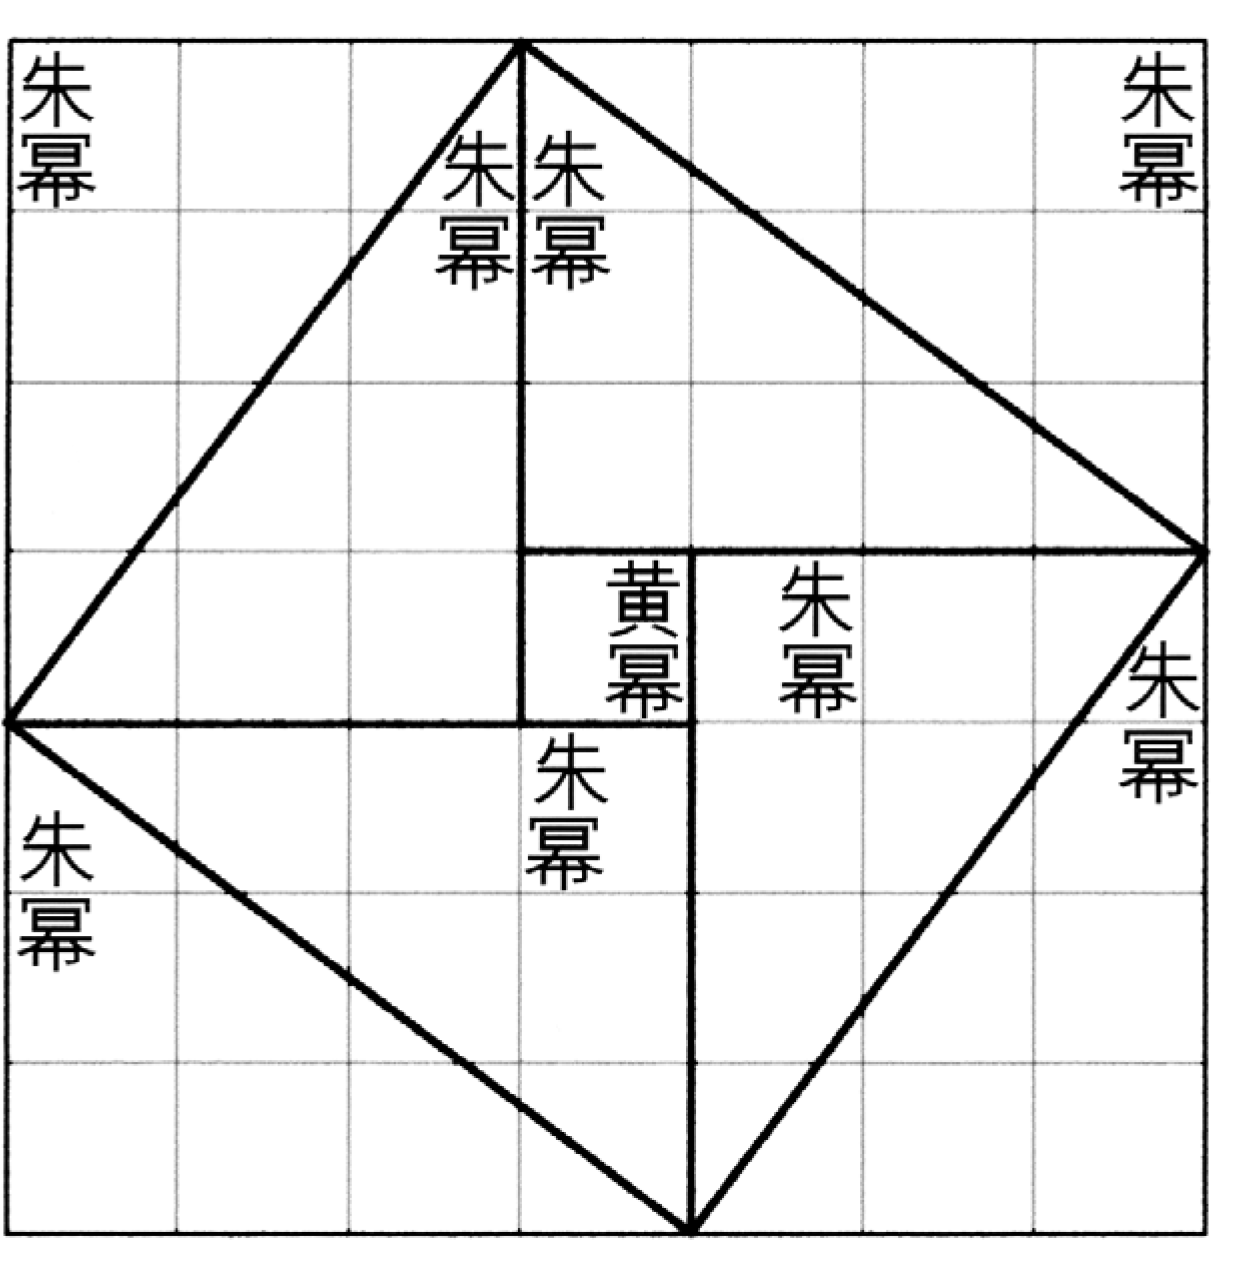
\includegraphics[width=3cm]{image_xiantu.png} 插入图片,但这种方式排版不好
\begin{figure}[ht]  % figure是插图使用的浮动体环境。可选参数[ht]表示浮动体可以出现在环境周围的文本所在处(here)和上一页的顶部(top)
    \centering  % 使其后的内容居中
    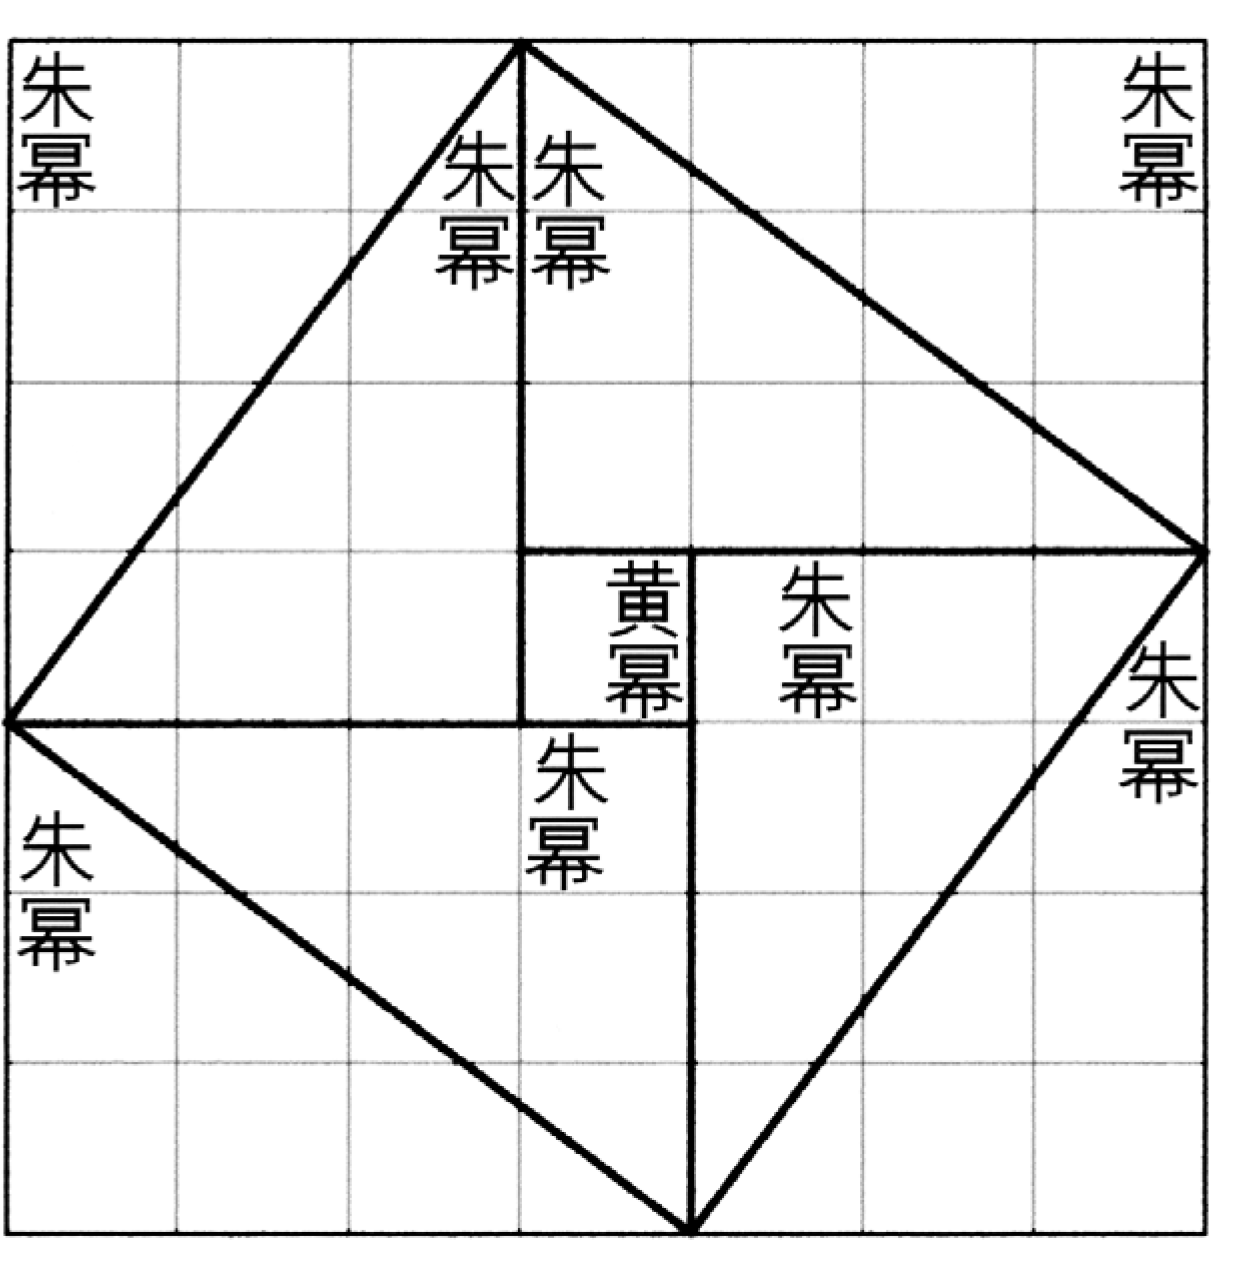
\includegraphics[scale=0.6]{image_xiantu.png}
    \caption{\zihao{-5}\kaishu 宋赵爽在《周髀算经》注中作的弦图(仿制),该图给出了勾股定理的一个极具对称美的证明\cite{quanjing}。} % caption命令给插图自动编号和加标题
    \label{fig:xiantu}  % 给图形定义一个标签,可以在其他地方使用这个标签引用|caption产生的编号
\end{figure}

\section{勾股定理的近代形式}
勾股定理可以用现代的语言表述如下:
\newtheorem{thm}{定理}
\begin{thm}[勾股定理]
    直角三角形斜边的平方等于两腰的平方和。

%    可以用符号的语言表述为:设直角三角形ABC,其中$\angle ACB = 90^\circ$,则有   % $\angle ACB = \pi / 2$,in-text formula or inline formula
可以用符号的语言表述为:设直角三角形ABC,其中$\angle ACB = 90\degree$,则有
\begin{equation}\label{eq:gougu}
    AB^2 = BC^2 + AC^2.
\end{equation}
\end{thm}
满足式\eqref{eq:gougu}的整数称为\emph{勾股数}。第\ref{sec:ancient}节所说的毕达哥拉斯学派得到的三元数组就是勾股数。下表列出一些较小的勾股数:
\begin{table}[H]   % 浮动环境table,格式与figure环境类似,只是\caption命令得到的标题是“表”而不是“图”。[H]参数设置来自包float,表示Hold,不浮动。

\begin{tabular}{|rrr|}  % tabular环境,|rrr|表示表格有三列,都是右对齐,第一列前和第三列后有竖线。r-right,l-left,c-center.
\hline  % 产生表格中的横线
直角边 $a$ & 直角边 $b$ & 斜边 $c$ \\   % 行与行之间用\\隔开
\hline
3 &  4 &  5 \\
5 & 12 & 13 \\
\hline
\end{tabular}%  % \end{tabular}后加一个%,用于取消换行产生的一个多余的空格
\qquad  % \qquad产生长为2em(大约两个“M”的宽度),将表格和公式隔开
($a^2 + b^2 = c^2$)
\end{table}

\nocite{Shiye}      % \nocite表示未直接引用的文献,一般放在\bibliography前面
\bibliography{math} % 从文献数据库math中获取文献信息,打印参考文献列表

\end{document}
